% ===== 原文 pp.51--54 =====

% [原文 p.51]
这里，矢量多重态的单圈行列式是对所有规范群因子的根 $\alpha$ 的乘积（即伴随表示的非零权）\footnote{准确地说，我们在此已把从整个规范代数 $\fg$ 上的积分转换到其 Cartan 子代数上时出现的 Vandermonde 行列式 $\prod_{\alpha\in\Delta}(\langle\alpha,ra\rangle)$ 包含进了 $Z^{\mathrm{vector}}_{\mathrm{one-loop}}$。}，
\begin{equation}
  Z^{\mathrm{vector}}_{\mathrm{one-loop}} = \prod_{\alpha\in\Delta}\Upsilon_b(\langle\alpha,ra\rangle),
  \tag{5.24}
\end{equation}
其中 $\Upsilon_b$ 是附录 A 中定义的特殊函数。我们强调，它在这里的宗量是纯虚的。超多重态的单圈行列式是对超多重态所变换的表示之权 $w$（带重数）的乘积，
\begin{equation}
  Z^{\mathrm{hyper}}_{\mathrm{one-loop}} = \prod_{w\in R}\frac{1}{\Upsilon_b\Big(\frac{b+1/b}{2}+\langle w,ra\rangle\Big)}.
  \tag{5.25}
\end{equation}
如前面所解释的，超多重态质量不过是与味对称性对应的矢量多重态标量的背景值，因此在 (5.25) 中加入质量 $m$ 只不过是把左端换成右端：
\begin{equation}
  \Upsilon_b\Big(\frac{b+1/b}{2}+\langle w,ra\rangle\Big)\to\Upsilon_b\Big(\frac{b+1/b}{2}+\langle w,ra\rangle+rm\Big).
  \tag{5.26}
\end{equation}

重要的是，表示 $R$ 与 $\bar R$ 中的超多重态是等价的（伴随 $m\to-m$），而借助对称性 $\Upsilon_b(b+1/b-x)=\Upsilon_b(x)$ 可以验证，用这两种表示算出的单圈行列式 (5.25) 相同。对于赝实表示 $R\simeq\bar R$ 中的半超多重态，每一对共轭权只应保留一个因子；由于 $\Upsilon_b$ 的同一对称性，每对中挑哪一个权并无区别。正如所预期的，由于 $\Upsilon_b=\Upsilon_{1/b}$，所有因子在 $S^4_b$ 的 $b\to1/b$ 对称性下不变。

% [Tutor Note: p.51 (5.25)--(5.26) 的自洽性核对：$\Upsilon_b(x)$ 的定义（附录 A）满足 $\Upsilon_b(b+1/b-x)=\Upsilon_b(x)$ 与 $\Upsilon_b=\Upsilon_{1/b}$。用 $\Upsilon_b(x)=1/(\Gamma_b(x)\Gamma_b(b+1/b-x))$ 立即可得第一条：把 $x\to b+1/b-x$ 只是交换两个 $\Gamma_b$ 因子。第二条则要求双 Gamma 函数在 $b\to1/b$ 下不变（其定义 $\Gamma_b(x)=\Gamma_2(x|b,b^{-1})/\Gamma_2(Q/2|b,b^{-1})$ 显然对称）。可用 $b=1$ 的退化情形作数值锚点：$\Upsilon_1(x)=1/(\Gamma_1(x)\Gamma_1(2-x))$，取 $x=1/2$ 得 $\Upsilon_1(1/2)=1/(\Gamma(1/2)\Gamma(3/2))=2/\pi$，与 $x\to 2-x$ 的对称性一致。另外 (5.26) 的质量平移 $+rm$ 说明 $rm$ 与 $\langle w,ra\rangle$ 同量纲，这也正是 $r$ 为球半径、$a,m$ 为标量期望值的体现。]

单圈行列式还可以进一步理解为来自南北两个半球的贡献之积，其本质是把每个 $\Upsilon_b$ 函数分解为 $\Upsilon_b(x)=1/(\Gamma_b(x)\Gamma_b(b+1/b-x))$。每个极点处的（反）瞬子只影响相应半球的单圈贡献，由此得到一个因子化性质，其形式为
\begin{equation}
  Z_{\mathrm{one-loop}}(a,k,\xi,\bar k,\bar\xi) = Z_{\mathrm{one-loop}}(a)Z_{\mathrm{one-loop,inst}}(a,k,\xi)Z_{\mathrm{one-loop,inst}}(a,\bar k,\bar\xi)
  \tag{5.27}
\end{equation}
其中 $\xi\in\cM_{G,k}$ 与 $\bar\xi\in\cM_{G,\bar k}$ 参数化瞬子构型，而 $Z_{\mathrm{one-loop}}(a)$ 就是上面写出的 $\Upsilon_b$ 之比值。

总之，把所有（反）瞬子贡献合到一起，并用 $q=\exp(2\pi\ii\tau)$ 表示经典贡献，配分函数可写为
\begin{equation}
  Z_{S^4_b} = \int \dd a\, Z_{\mathrm{cl}}(a,q\bar q)Z_{\mathrm{one-loop}}(a)Z_{\mathrm{inst}}(a,q)Z_{\mathrm{inst}}(a,\bar q).
  \tag{5.28}
\end{equation}
这里，积分遍历所有规范群的 Cartan 代数，$Z_{\mathrm{one-loop}}$ 如上给出，而 $Z_{\mathrm{cl}}=\exp(-S_{\mathrm{cl}})=|q|^{r^2|a|^2}$ 中的指数涉及李代数的 Killing 型 $|a|^2=-\Tr(a^2)$，由于 $a$ 是虚的，它是正的。

% [原文 p.52]
我们把瞬子对 $S_{\mathrm{cl}}$ 的修正收进 $Z_{\mathrm{inst}}$，并把 $Z_{\mathrm{one-loop,inst}}$ 适当地在瞬子模空间上积分：
\begin{equation}
  Z_{\mathrm{inst}}(a,q) = \sum_{\text{所有 }k_I\ge 0}\Big(\prod_I q_I^{k_I}\Big)\int_{\prod_I\cM_{G_I,k_I}}Z_{\mathrm{one-loop,inst}}(a,k,\xi)\,\dd\xi.
  \tag{5.29}
\end{equation}
剩下的就是计算这个瞬子配分函数。

\subsection{瞬子配分函数}

\para{Omega 背景。} (5.19) 中的点状构型只对超引力背景在极点附近的领头展开敏感。这个超引力背景具有平坦度规和非平凡的引力光子（graviphoton），并且与 Nekrasov [12] 发现的 Omega 背景 $\R^4_{\epsilon_1,\epsilon_2}$ 一致，其参数为 $\epsilon_1=b/r$、$\epsilon_2=1/(rb)$。因此人们自然地猜想 [10, 11]（以及后续工作）：在 $Z_{S^4_b}$ 的表达式 (5.28) 中，所应纳入的函数 $Z_{\mathrm{inst}}(a,q)=1+O(q^1)$ 正是该 4d $\cN=2$ 理论在 Omega 背景 $\R^4_{\epsilon_1,\epsilon_2}$ 上的配分函数，称为 Nekrasov 瞬子配分函数 [12, 13]。关于 $Z_{\mathrm{inst}}$ 的更详细介绍可参见综述 [116, 127]。

当 $\epsilon_1,\epsilon_2\to 0$ 时 Omega 背景趋于 $\R^4$，因此可把它理解为因 $\R^4$ 非紧而生的红外发散的正则化手段。事实上，如 [12, 13] 以及 [193] 的附录中所解释的，该配分函数给出规范理论的低能预势\footnote{预势是 $\cN=2$ 超空间中的拉格朗日密度，它完全编码了 Coulomb 分支一般点上 U(1) 规范场的低能动力学。关于这个关键函数的更多讨论可参见 [115] 等综述。}：
\begin{equation}
  F(a,q) = F_{\mathrm{pert}}(a,q) + \lim_{\epsilon_1,\epsilon_2\to 0}\Big(\epsilon_1\epsilon_2\log Z_{\mathrm{inst}}(a,q;\epsilon_1,\epsilon_2)\Big),
  \tag{5.30}
\end{equation}
其中 $F_{\mathrm{pert}}$ 来自单圈计算，可由 $Z_{\mathrm{one-loop}}$ 提取。这样一来，瞬子配分函数就给出了 4d $\cN=2$ 理论在 Coulomb 分支上一点 $a$ 处的低能动力学的信息。整条 Seiberg--Witten 曲线随后可以被严格地导出，如 [13, 194, 195] 所做的那样。该推导依赖于与随机分拆（random partitions）理论的联系。

% [Tutor Note: p.52 参数锚点：$\epsilon_1=b/r$、$\epsilon_2=1/(rb)$ 给出 $\epsilon_1\epsilon_2=1/r^2$，因此 (5.30) 中 $\epsilon_1\epsilon_2\log Z_{\mathrm{inst}}$ 的量纲正确（$\log Z$ 无量纲，$1/r^2$ 与预势中标量场的平方同量纲）。与 (5.28) 的经典项对照：按定义 $|a|^2=-\Tr(a^2)$，故 $\Tr(ra)^2=-r^2|a|^2$，可见 $r^2|a|^2$ 就是 $-\Tr(ra)^2$；再结合 (5.22) 的 $S_{\mathrm{cl}}=-\Re(2\pi\ii\tau)\Tr(ra)^2+\cdots$，$Z_{\mathrm{cl}}$ 的指数正是 $\Re(2\pi\ii\tau)r^2|a|^2$ 的幅度，两式自洽。另外 $\epsilon_1/\epsilon_2=b^2$ 与 $S^4_b$ 的压扁参数 $b$ 对应，这解释了为什么 $b\to1/b$ 对称性在 $\epsilon_1\leftrightarrow\epsilon_2$ 交换下成立。]

Omega 背景也可以作为 5d 背景 $S^1_\beta\times_{\epsilon_1,\epsilon_2}\R^4$ 的 $\beta\to0$ 极限得到，后者定义为 $\R\times\C\times\C$ 在等价关系 $(x,z_1,z_2)\sim(x+\beta,\ee^{\ii\beta\epsilon_1}z_1,\ee^{\ii\beta\epsilon_2}z_2)$ 下的商。许多 4d $\cN=2$ 拉格朗日理论可以提升为 5d $\cN=1$ 理论，此时瞬子配分函数 $Z_{\mathrm{inst}}$ 有 5d 的对应物，即定义为在 $S^1_\beta\times_{\epsilon_1,\epsilon_2}\R^4$ 上的配分函数。此外还值得一提关于如何在弦论与 M 理论中构造 Omega 背景的进展 [196--200]。

\para{计算方法。} 瞬子配分函数是瞬子模空间上的积分，其被积函数依赖于物质。如上所述，该模空间按单规范群因子分解为乘积，而每个规范群因子的模空间对每个瞬子数 $k\ge0$ 有一个连通分支，维数随 $k$ 增长。计算瞬子配分函数有若干种方法 [127]\footnote{感谢 Jaewon Song 就某些方法所作的通信。}。

% [原文 p.53]
\begin{itemize}[leftmargin=1.4em,itemsep=2pt,topsep=2pt]
\item
\para{ADHM 构造。} 对于经典规范群 U（而非 SU）、USp、SO，$n$-瞬子模空间可以通过 Atiyah--Drinfeld--Hitchin--Manin（ADHM）构造实现为辛商 [201]；而对于例外群 $E_6,E_7,E_8,F_4,G_2$ 以及 SU，一般而言并没有这类构造。在物理上，ADHM 构造把瞬子模空间表示为某个超对称矩阵模型的模空间，该矩阵模型描述 D3 膜与 O3 平面背景中的 D$(-1)$ 膜瞬子，而这些膜实现 4d $\cN=2$ 矢量多重态 [202--204]。该矩阵模型对处于合适表示（如双基本表示）的超多重态是已知的。局域化随后把 $Z_{\mathrm{inst}}$ 从整个模空间上的积分约化为一个离散求和，求和项来自保持某些 U(1) 对称性的点状瞬子集合的贡献。我们在下文 (5.33) 中给出 U($N$) 规范理论的结果公式。这个 Losev--Moore--Nekrasov--Shatashvili（LMNS）公式由 [205--207] 得到、由 [12] 导出，并被推广到其他经典群 [208--210]、箭图 [194] 以及超群理论 [211]。这些方法适用于这些理论的 5d $\cN=1$ 提升：$S^1_\beta\times_{\epsilon_1,\epsilon_2}\R^4$ 上的瞬子配分函数与矩阵模型之量子力学类比的超对称指标相吻合（例如见 [212, 213]）。

\item
\para{纯 4d $\cN=2$ SYM。} 对于例外规范群没有 ADHM 构造。单瞬子模空间是（$\C^2$ 乘以）$G$ 作用在其余伴随表示最高权向量上的轨道。这使得任意规范群的纯 SYM 单瞬子配分函数可以用群论方法计算 [99, 214, 215]。这一计算在 [216] 中被推广到双瞬子。

与 ADHM 构造中把 $k$-瞬子模空间实现为 Higgs 分支不同，它也可以实现为某个 3d $\cN=4$ SCFT 的 Coulomb 分支。这个 3d 理论的 Coulomb 分支 Hilbert 级数（超共形指标的一个特殊化）随即给出任意规范群的纯 SYM 在 $S^1_\beta\times_{\epsilon_1,\epsilon_2}\R^4$ 上的 $k$-瞬子配分函数 [217]。纯 $E_n$ SYM 理论的瞬子配分函数可以由 $E_n$ Minahan--Nemeschansky 理论的 Hall--Littlewood 指标确定，而后者可用 9.2 小节讨论的 TQFT 实现来计算。

\item
\para{质量形变的 4d $\cN=4$ SYM。} 对于 4d $\cN=2^*$ SYM（它随质量变化在 $\cN=4$ 与 $\cN=2$ SYM 之间插值），预势（或它的 Omega 形变）被期望满足一个模反常方程，该方程描述它在 S 对偶下如何变换 [218, 219]。这导向了用 Eisenstein 级数表示任意规范群预势的公式 [220--223]。这一技巧在一定程度上有推广，例如推广到共形 SQCD [224, 225]。
\end{itemize}

% [原文 p.54]
\begin{itemize}[leftmargin=1.4em,itemsep=2pt,topsep=2pt]
\item
\para{递推关系。} 把瞬子配分函数与 $\C^2$ 爆破（blow-up）上的配分函数作比较，可得到递推关系（见 [226--228] 及其中的参考文献）。对于经典规范群与例外规范群的一大类表示中的超多重态（但不含半超多重态），可以求解这些递推关系，并从微扰（单圈）配分函数推出 $Z_{\mathrm{inst}}$。
\end{itemize}

有些物质表示逃出了所有可用的方法：最值得注意的是由 SU(2) 矢量多重态与三基本表示半超多重态构造的一般拉格朗日量，它们正是 SU(2) class S 理论的拉格朗日描述。在这些理论中，只要能用规范群 SU(2) 与 SO(4) $=(\mathrm{SU}(2)\times\mathrm{SU}(2))/\Z_2$ 以及双基本表示物质（两个 SU(2) 群的，或一个 SU(2) 群与一个 SO(4) 群的）写出该理论，$Z_{\mathrm{inst}}$ 就是已知的；见 [96, 98]。一个可能的出路依赖于拓扑顶点形式 [229]。

Nekrasov 配分函数有许多推广，例如在 ALE 空间 [82, 230--235] 和更一般的空间 [236--238] 上、尖刺型瞬子（spiked instantons）[239]，以及一个关于 4d $\cN=1$ 理论的推广提议 [240]。

\para{线性箭图规范理论的显式公式。} 现在我们关注线性箭图规范理论
\begin{equation}
  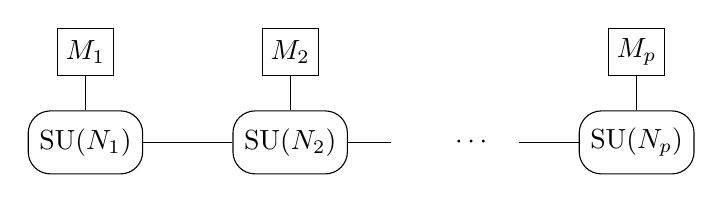
\begin{tikzpicture}[baseline=(current bounding box.center)]
    \node[draw, rounded corners=8pt, inner sep=4pt, minimum height=8mm] (n1) at (0,0) {$\mathrm{SU}(N_1)$};
    \node[draw, rounded corners=8pt, inner sep=4pt, minimum height=8mm] (n2) at (2.6,0) {$\mathrm{SU}(N_2)$};
    \node[draw, rounded corners=8pt, inner sep=4pt, minimum height=8mm] (np) at (7.0,0) {$\mathrm{SU}(N_p)$};
    \node[draw, inner sep=3pt, minimum height=6mm] (m1) at (0,1.15) {$M_1$};
    \node[draw, inner sep=3pt, minimum height=6mm] (m2) at (2.6,1.15) {$M_2$};
    \node[draw, inner sep=3pt, minimum height=6mm] (mp) at (7.0,1.15) {$M_p$};
    \draw (m1.south) -- (n1.north);
    \draw (m2.south) -- (n2.north);
    \draw (mp.south) -- (np.north);
    \draw (n1.east) -- (n2.west);
    \draw (n2.east) -- ++(0.55,0);
    \node at (4.9,0) {$\cdots$};
    \draw (5.5,0) -- (np.west);
  \end{tikzpicture}
  \tag{5.31}
\end{equation}
它是 4.4 小节中那些理论的一个轻微推广（允许 $N_i$ 互不相同）。该理论的规范群为 $\prod_{i=1}^{p}\mathrm{SU}(N_i)$，每个双基本表示 $N_i\otimes N_{i+1}$ 中有一个超多重态，而每个群的 $M_i$ 个超多重态按基本表示 $N_i$ 变换。若该理论是共形的或渐近自由的，即贝塔函数系数 $b_j=2N_j-N_{j-1}-N_{j+1}-M_j$ 非负，则它可以借助箭图尾巴在 class S 中实现，见 (7.15)。

% [Tutor Note: p.54 (5.31) 原文是一个箭图（示意图），已按 STYLE_GUIDE §6bis 用 TikZ 重画：圆角矩形为规范群节点 $\mathrm{SU}(N_i)$，上方方框为该节点上的基本超多重态数目 $M_i$，水平连线为双基本表示 $N_i\otimes N_{i+1}$。核对要点：$\beta$ 函数系数 $b_j=2N_j-N_{j-1}-N_{j+1}-M_j$ 正好是 4d SU($N$) 规范理论的单圈系数（矢量 $-2N$、每个双基本 $+1$、每个基本 $+1$，再取反号），$b_j\ge0$ 即渐近自由或共形；这也解释了 (7.15) 中 class S 的箭图尾巴实现为何要求 $b_j\ge0$。]

把规范群从 SU($N_i$) 推广到 U($N_i$) 后，该理论可以在 IIA 弦论中实现：它是若干组 $N_i$ 个平行 D4 膜的世界体理论，这些 D4 膜伸展在相邻 NS5 膜之间，此外还有 $M_i$ 个横向 D6 膜，它们给出基本超多重态，如图 3 所示。瞬子被描述为同样伸展在 NS5 膜之间的 D0 膜，而 $Z_{\mathrm{inst}}$ 就是它们世界体理论的配分函数，并对 D0 膜的数目求和。最终必须除掉由额外 U(1) 规范群造成的多余因子。

% [Tutor Note: p.54 末段与 p.56 (5.35)：把 D4 膜的数目 $N_i$ 所对应的 SU($N_i$) 扩成 U($N_i$) 会多出一个“对角”U(1)，它不对应膜上的独立自由度，因此必须除掉 (5.35) 中的 U(1) 因子。可核对的锚点：$b_j=0$（共形）时 $z_j\simeq\ee^{2\pi\ii\tau_j}$，而 $b_j>0$（渐近自由）时 $z_j=\Lambda_j^{b_j}$（见 p.55 脚注 45），这正是 4d 瞬子计数参数与动力学能标的两种标准关系。]

我们记 Coulomb 分支参数为 $a^i=\{a^i_1,\dots,a^i_{N_i}\}$（$1\le i\le p$），并记 $k_i$ 为 U($N_i$) 的瞬子数，即第 $i$ 个 NS5 膜间区间中 D0 膜的数目。于是
\begin{equation}
  Z_{\mathrm{inst}}\Big[\prod \mathrm{U}(N_i)\Big] = \sum_{k_1\ge0,\dots,k_p\ge0} z_1^{k_1}\cdots z_p^{k_p}\, Z^{(k)}_{\mathrm{inst}},
  \tag{5.32}
\end{equation}
其中计数参数 $z_j$ 编码第 $j$ 个规范群的动力学能标 $\Lambda_j$ 或规范耦合 $\tau_j$\footnote{若 $b_j=2N_j-N_{j-1}-N_{j+1}-M_j$ 为正，则 $z_j=\Lambda_j^{b_j}$；而若 $b_j=0$，则 $z_j$ 本质上就是 $\ee^{2\pi\ii\tau_j}$。准确地说，“$\tau_j$ 指什么”存在若干重整化方案的含混，我们马上会在第 56 页讨论。更合理的逻辑是：从 $Z_{\mathrm{inst}}$ 提取作为 $z_j$ 函数的预势，推出红外耦合与 $z_j$ 的关系，最后若想用物理上有意义的量表示 $z_j$，再把这个映射反过来。}。
